\chapter{نتایج}

در این فصل سعی شده است تا با ارائه تعدادی تصاویر از محیط سامانه و عملکرد آن، خروجی سامانه و همچنین برخی از آزمون‌های تولید شده نیز ارائه شود. البته تعداد بسیار بیشتری تصویر و بخش قابل ارائه بود اما در این‌صورت حجم این گزارش بسیار زیاد می‌شد. همچنین  بدلیل این‌که جزئیات کار سامانه در فصول قبلی شرح داده شده از توضیح تصاویر فوق صرف‌نظر شده است.

%\section{سامانه اصلی}

%\subsection{ساختار فایل‌ها}

\begin{figure}[H]
	\centering
	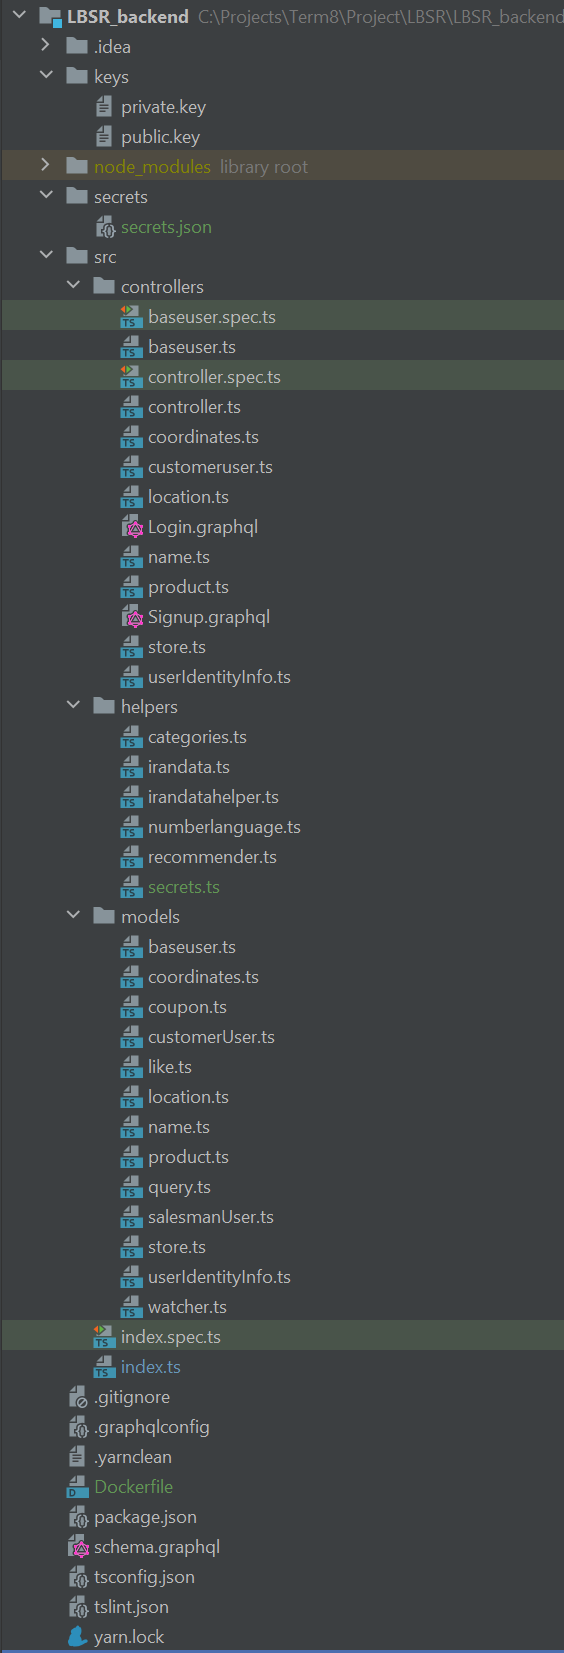
\includegraphics[scale=0.5]{files}
	\caption{فایل‌های سامانه اصلی}
	\label{fig:files}
\end{figure}

%\subsection{خروجی سامانه اصلی}

در خروجی سامانه اصلی یک سرویس تحت وب ارائه می‌شود که شامل \lr{API}های سامانه و یک محیط تست و بررسی آن‌ها (تحت عنوان \lr{Apollo Playground}) است. در \cref{fig:backend} این محیط قابل مشاهده است.

\begin{figure}[H]
	\centering
	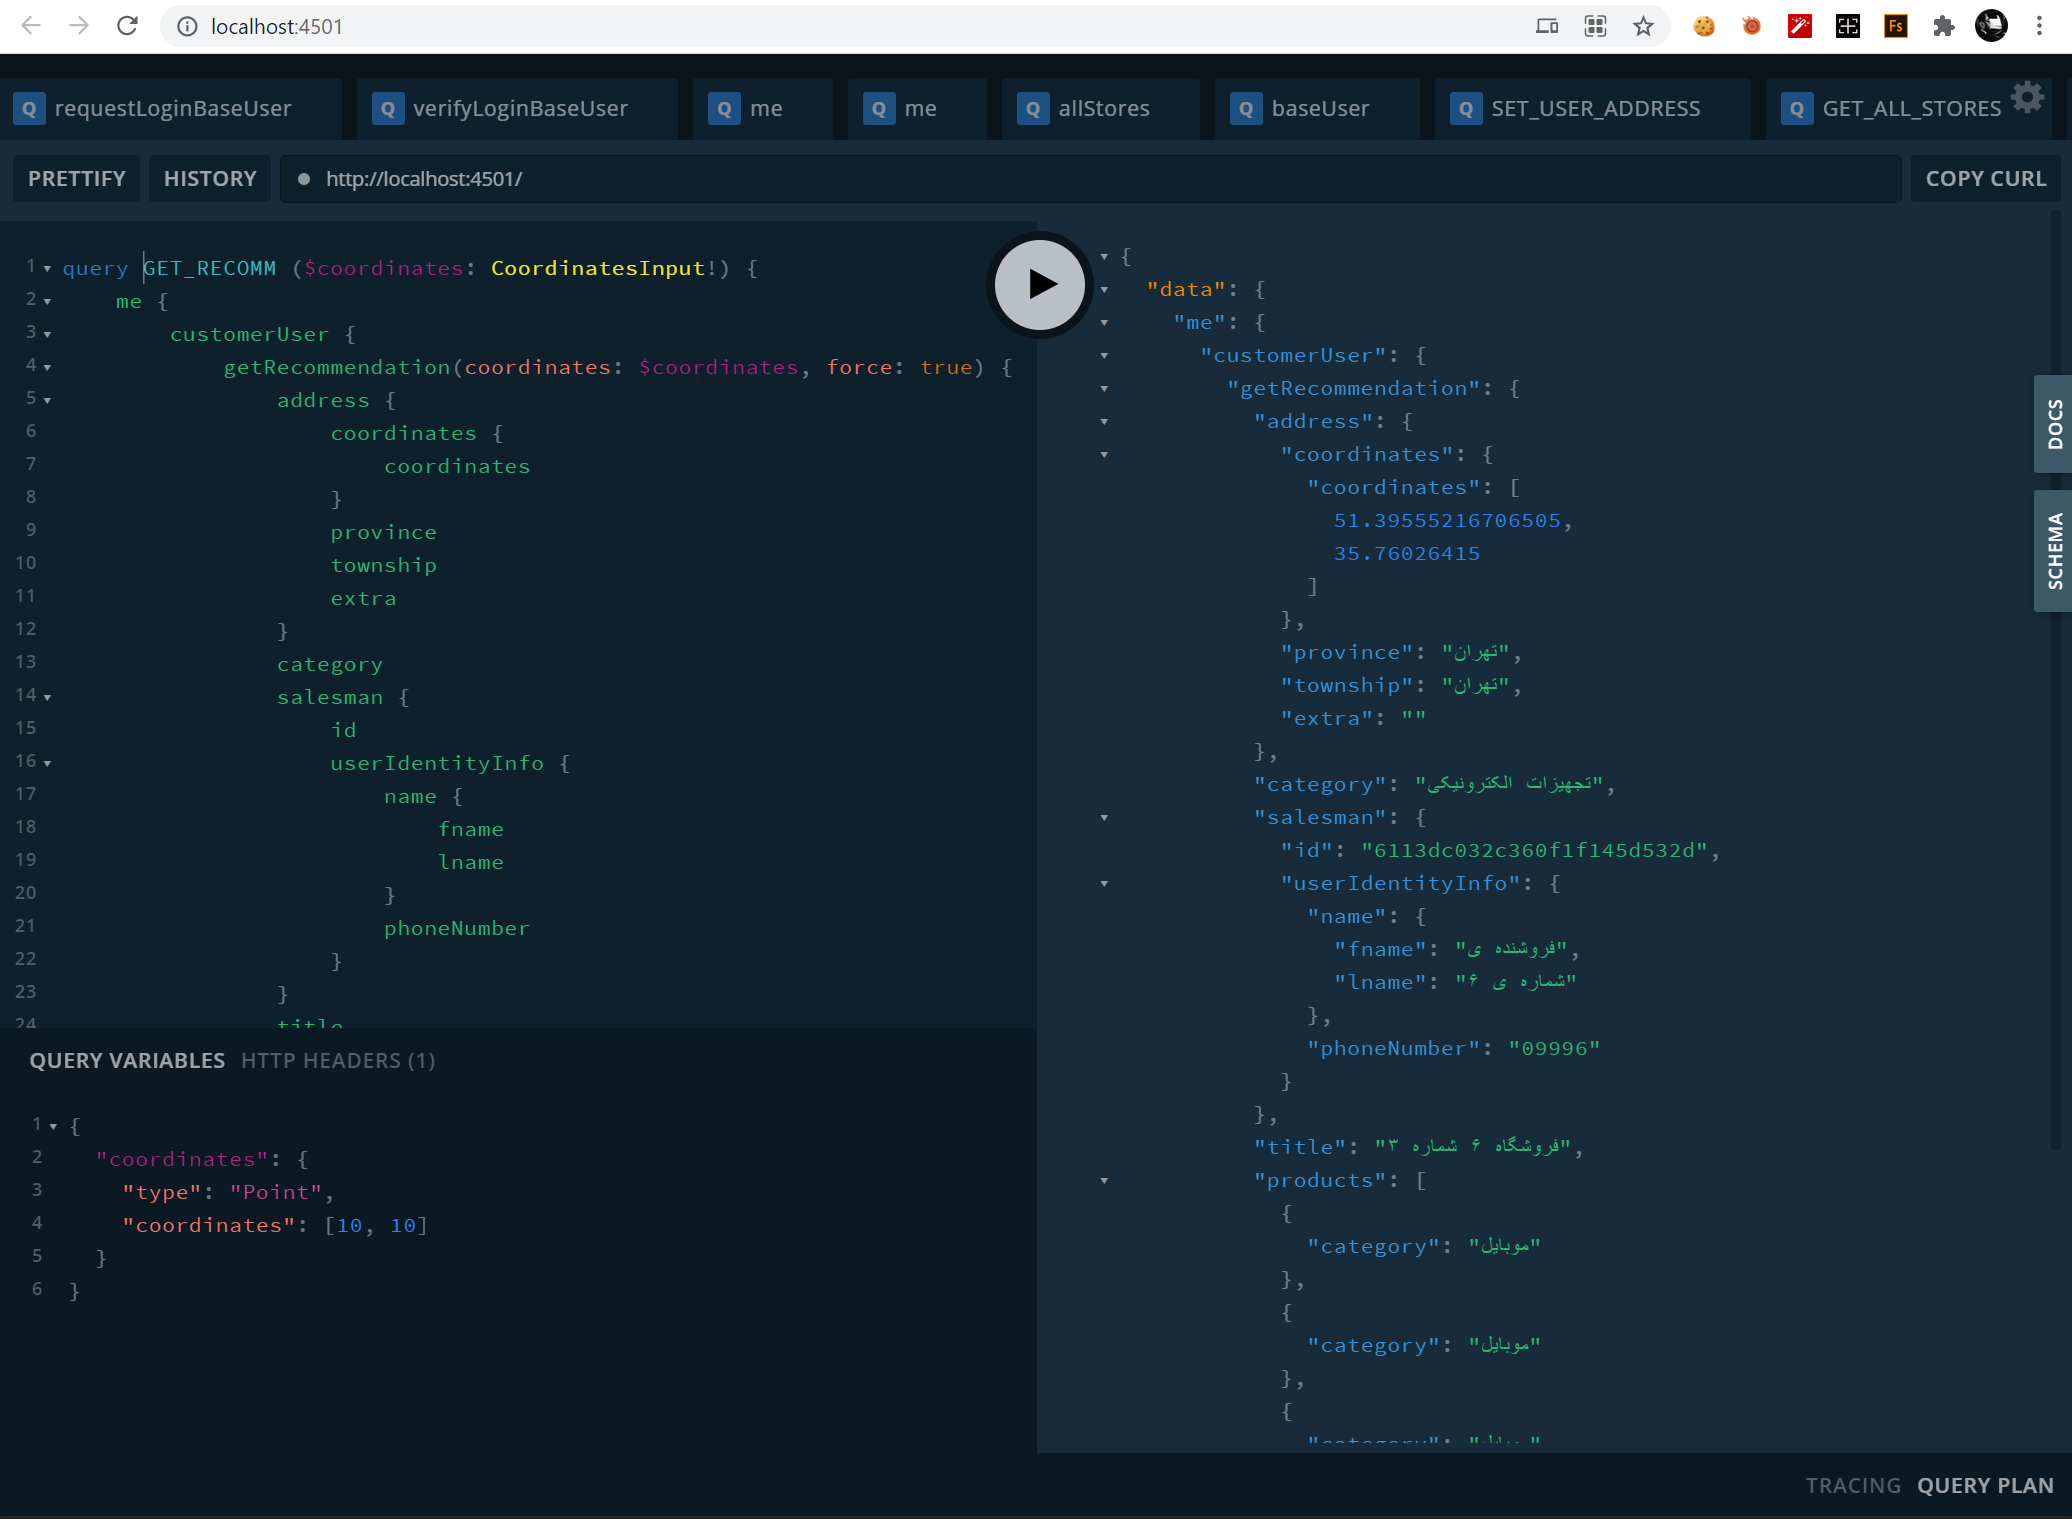
\includegraphics[scale=0.45]{backend}
	\caption{درخواست ازمایشی دریافت پیشنهاد مبتنی بر مکان}
	\label{fig:backend}
\end{figure}

همچنین در \cref{fig:api1}، بخشی از رابط برنامه‌نویسی کاربردی ارائه شده توسط سامانه اصلی (تحت استاندارد گرف‌کیوال) قابل مشاهده است که در ادامه به توضیح گره‌های مهم‌تر موجود در این ساختار خواهیم پرداخت.


\begin{enumerate}
	\item \lr{requestLoginBaseUser}: این گره برای درخواست اولین مرحله از فرآیند ورود/ثبت‌نام اجرا می‌شود که در نتیجه آن، کد تایید ورود به شماره داده شده پیامک خواهد شد.
	\item \lr{verifyLoginBaseUser}: این گره ادامه فرایند ورود/ثبت‌نام را انجام می‌دهد و درصورت صحت کد تایید (که به همراه شماره موبایل ورودی داده می‌شود) بلیت جدیدی توسط \lr{JWT} ایجاد شده و در خروجی ارسال می‌شود.
	\item \lr{allStores}: از این گره برای دریافت لیست فروشگاه‌ها استفاده می‌شود که در دو قسمت کاربرد دارد؛ اولین کاربرد آن در صفحه اصلی نرم‌افزار موبایل هوشمند است و کاربرد دوم آن در پنل مدیران. اگر از طریق پنل مدیران اجرا شود، باید مقداری تحت عنوان \lr{AdminMasterPassword} که یک توصیف امنیتی قراردادی بین سامانه اصلی و پنل مدیران است در پارامترهای ورودی آن ارسال شود.
	\item \lr{allUsers}: این گره لیست تمام کاربران را بازمی‌گرداند و فقط در پنل مدیران استفاده شده است و مانند مورد قبل برای اجرا به توصیف امنیتی گفته شده احتیاج خواهد داشت.
	\item \lr{me}: این گره برای دسترسی به خصوصیات و توابع کاربر فعلی است. برای اجرای این گره حتما باید سرآیند \lr{Authorization} در درخواست ورودی با مقدار صحیحی از بلیت \lr{JWT} تنظیم شده باشد.
	\item \lr{baseUser}: این گره برای دسترسی به اطلاعات کاربران دیگر است. برای این‌که مجوز چنین دسترسی‌ای وجود داشته باشد، کاربر هدف باید بعنوان فروشنده تعریف شده باشد. آی‌دی کاربر هدف در تنها پارامتر این گره داده می‌شود.
\end{enumerate}

تمامی جزئیات بعدی درون تایپ \lr{BaseUser} قرار گرفته‌اند که در پاسخ به درخواست \lr{me} و یا \lr{baseUser} بازگردانده می‌شود. بطور مختصر، درون این تایپ گره‌های زیر قرار دارند:

\begin{enumerate}
	\item \lr{id}: آی‌دی کاربر،
	\item \lr{userIdentityInfo}: شئ شامل اطلاعات هویتی و شخصی کاربر از جمله نام، شماره موبایل و آدرس،
	\item \lr{isSalesman}: یک پرچم\footnote{\lr{Flag}} که نوع کاربر را مشخص می‌کند و اگر مقدار آن \lr{true} باشد به معنای فروشنده بودن این کاربر است،
	\item \lr{customerUser}: برای تمامی کاربران تعریف شده و شامل گره‌های زیر می‌شود:
	\begin{enumerate}
		\item \lr{locations}: آرایه‌ای از موقعیت‌های مکانی دوره‌ای ثبت شده از کاربر را برمی‌گرداند که می‌تواند برای تحلیل‌های بعدی مورد استفاده قرار بگیرد،
		\item \lr{addCoordinates}: برای ثبت موقعیت‌های مکانی دوره‌ای کاربر استفاده می‌شود و یک موقعیت جدید را ثبت می‌کند،
		\item \lr{getRecommendation}: این گره بخش اصلی کار ارائه پیشنهاد را انجام می‌دهد و با محاسبه علاقه‌مندی‌های کاربر و دریافت موقعیت مکانی فعلی او، یک فروشگاه را بعنوان نزدیک‌ترین پیشنهاد بازمی‌گرداند،
	\end{enumerate}
	\item \lr{salesmanUser}: این گره فقط برای فروشندگان تعریف شده و شامل گره‌های زیر می‌شود:
	\begin{enumerate}
		\item \lr{setStores, addStore, removeStore, editStore}: این گره‌ها برای اضافه، حذف و تغییر فروشگاه و یا فروشگاه‌های یک فروشنده استفاده می‌شوند،
		\item \lr{stores}: لیست کل فروشگاه‌های این فروشنده را باز می‌گرداند،
		\item \lr{store}: این گره با دریافت نام و دسته‌بندی فروشگاه، شئ آن فروشگاه را برمی‌گرداند. هر فروشگاه شامل گره‌های زیر می‌شود:
		\begin{enumerate}[label=\arabic*.]
			\item \lr{title}: نام فروشگاه،
			\item \lr{category}: دسته‌بندی فروشگاه،
			\item \lr{setProducts, addProduct, removeProduct, editProduct}: این گره‌ها برای اضافه، حذف و تغییر محصول و یا محصولات یک فروشگاه استفاده می‌شوند،
			\item \lr{products}: لیست کل محصولات این فروشگاه را باز می‌گرداند،
			\item \lr{product}: این گره با دریافت نام و زیردسته‌ی محصول، شئ آن محصول را برمی‌گرداند. هر محصول شامل گره‌های زیر می‌شود:
			\begin{enumerate}
				\item \lr{title}: نام محصول،
				\item \lr{category}: زیردسته‌ی محصول،
				\item \lr{description}: توضیحات محصول،
				\item \lr{coupons}: لیست کوپن‌های محصول،
				\item \lr{likes}: لیست علاقه‌مندی‌های اعلام شده به این محصول،
				\item \lr{watchers}: لیست زیرنظرگرفتن‌های محصول،
				\item \lr{remainingCouponsCount}: تعداد کوپن‌های باقیمانده،
				\item \lr{likesCount}: تعداد علاقه‌مندی‌های اعلام شده،
				\item \lr{watchersCount}: تعداد زیرنظرگرفتن‌ها،
				\item \lr{isLikedByMe}: این گره درصورتی که کاربر درخواست‌دهنده به حسابش وارد شده باشد، وضعیت اعلام علاقه‌مندی او را نسبت به این محصول مشخص می‌کند،
				\item \lr{isWatchedByMe}: این گره نیز مانند گره قبلی برای زیرنظرگرفتن محصولات است،
				\item \lr{canIGetCoupon}: همانند دو گره قبلی،‌این گره بیان می‌کند که آیا کاربر فعلی می‌تواند کوپن دیگری را از این محصول دریافت کند یا خیر (فارغ از این‌که قبلا کوپنی دریافت کرده باشد)،
				\item \lr{like}: اگر کاربر به حساب کاربری‌اش وارد شده باشد، می‌تواند با این گره محصول را به علاقه‌مندی‌های خودش اضافه کند،
				\item \lr{watch}: مانند گره قبلی است، ولی به لیست زیرنظرگرفته‌شده‌ها اضافه می‌شود،
				\item \lr{unlike}: برای حذف محصول از لیست علاقه‌مندی،
				\item \lr{unwatch}: برای حذف محصول از لیست زیرنظرگرفته‌شده‌ها،
				\item \lr{getCoupon}: اگر کاربر به حساب خودش وارد شده باشد، با این گره می‌تواند درخواست دریافت یک کد تخفیف (کوپن) بدهد،
				\item \lr{gottenCoupons}: اگر کاربر وارد شده باشد، با این گره می‌تواند به لیست کوپن‌های دریافتی قبلی دسترسی پیدا کند،
				\item \lr{addCoupon}: صاحب این فروشگاه می‌تواند با این گره به این محصول کدهای تخفیف اضافه کند،
				\item \lr{storeTitle}: نام فروشگاه محصول،
				\item \lr{storeCategory}: دسته‌بندی فروشگاه محصول.	
				
			\end{enumerate}
		\end{enumerate}
	\end{enumerate}
\end{enumerate}


\begin{figure}[H]
	\centering
	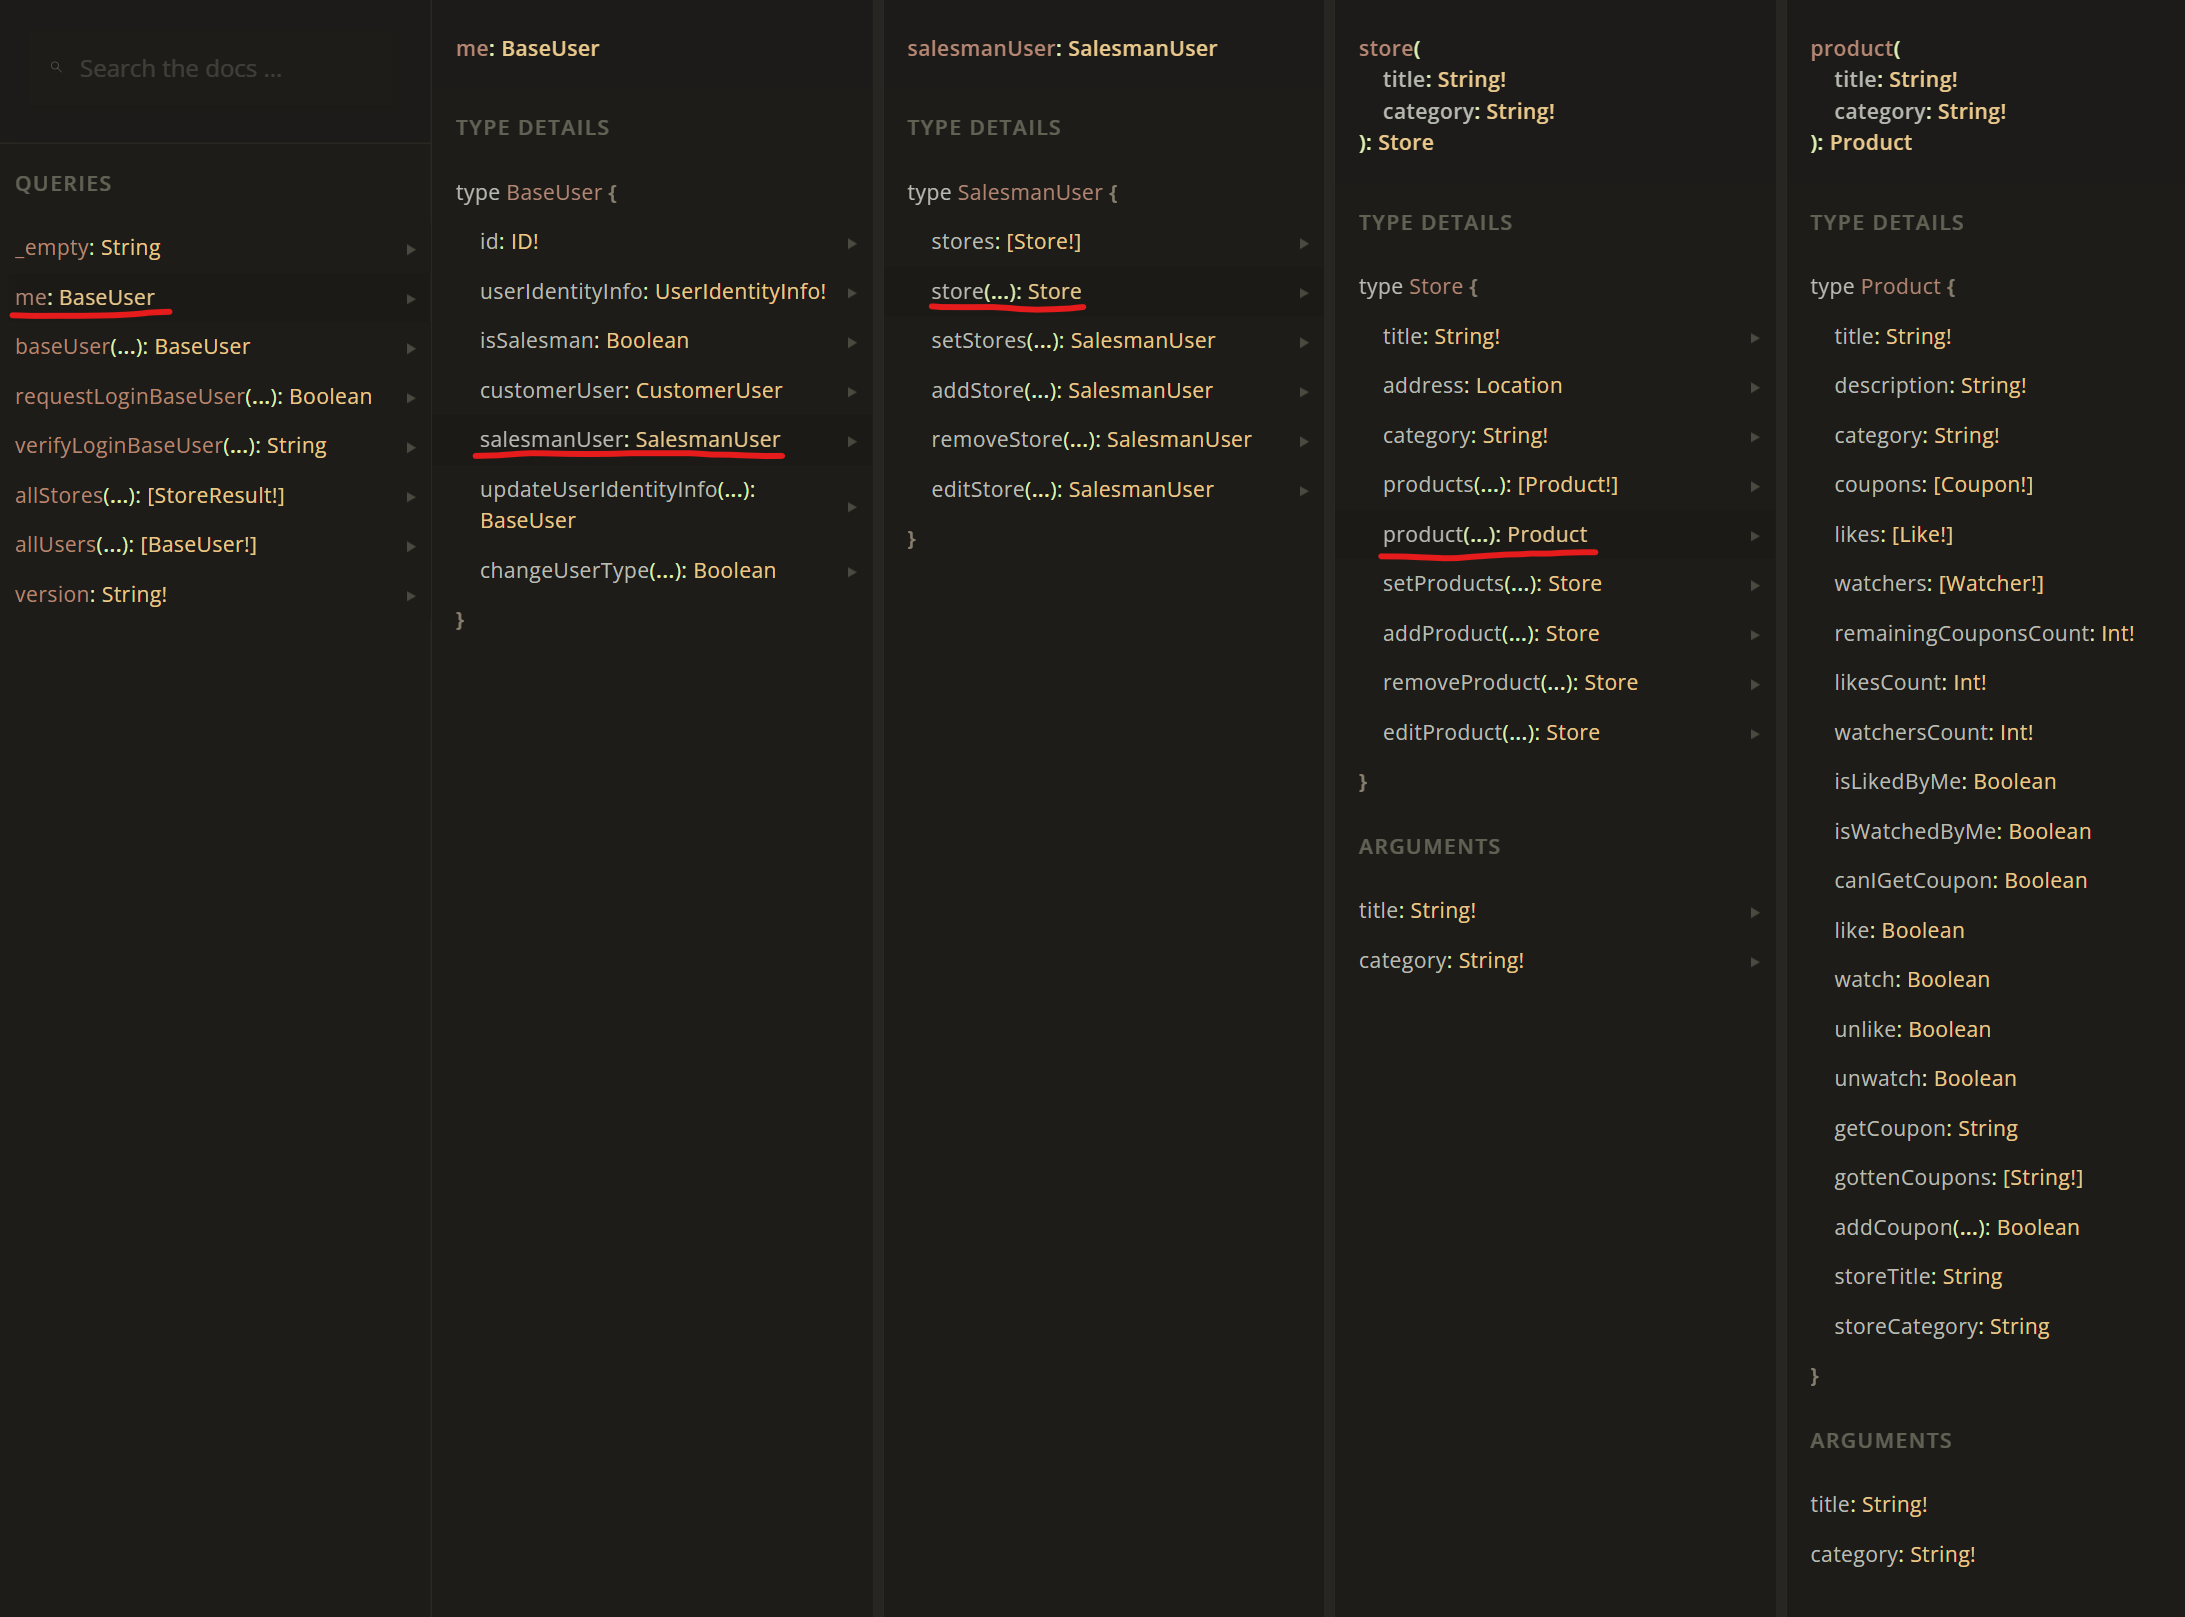
\includegraphics[scale=0.4]{api1}
	\caption{بخشی از \lr{API} ارائه شده توسط سامانه اصلی}
	\label{fig:api1}
\end{figure}




\newpage

%\subsection{خروجی نرم‌افزار کاربردی}

\begin{figure}[H]
	\centering
	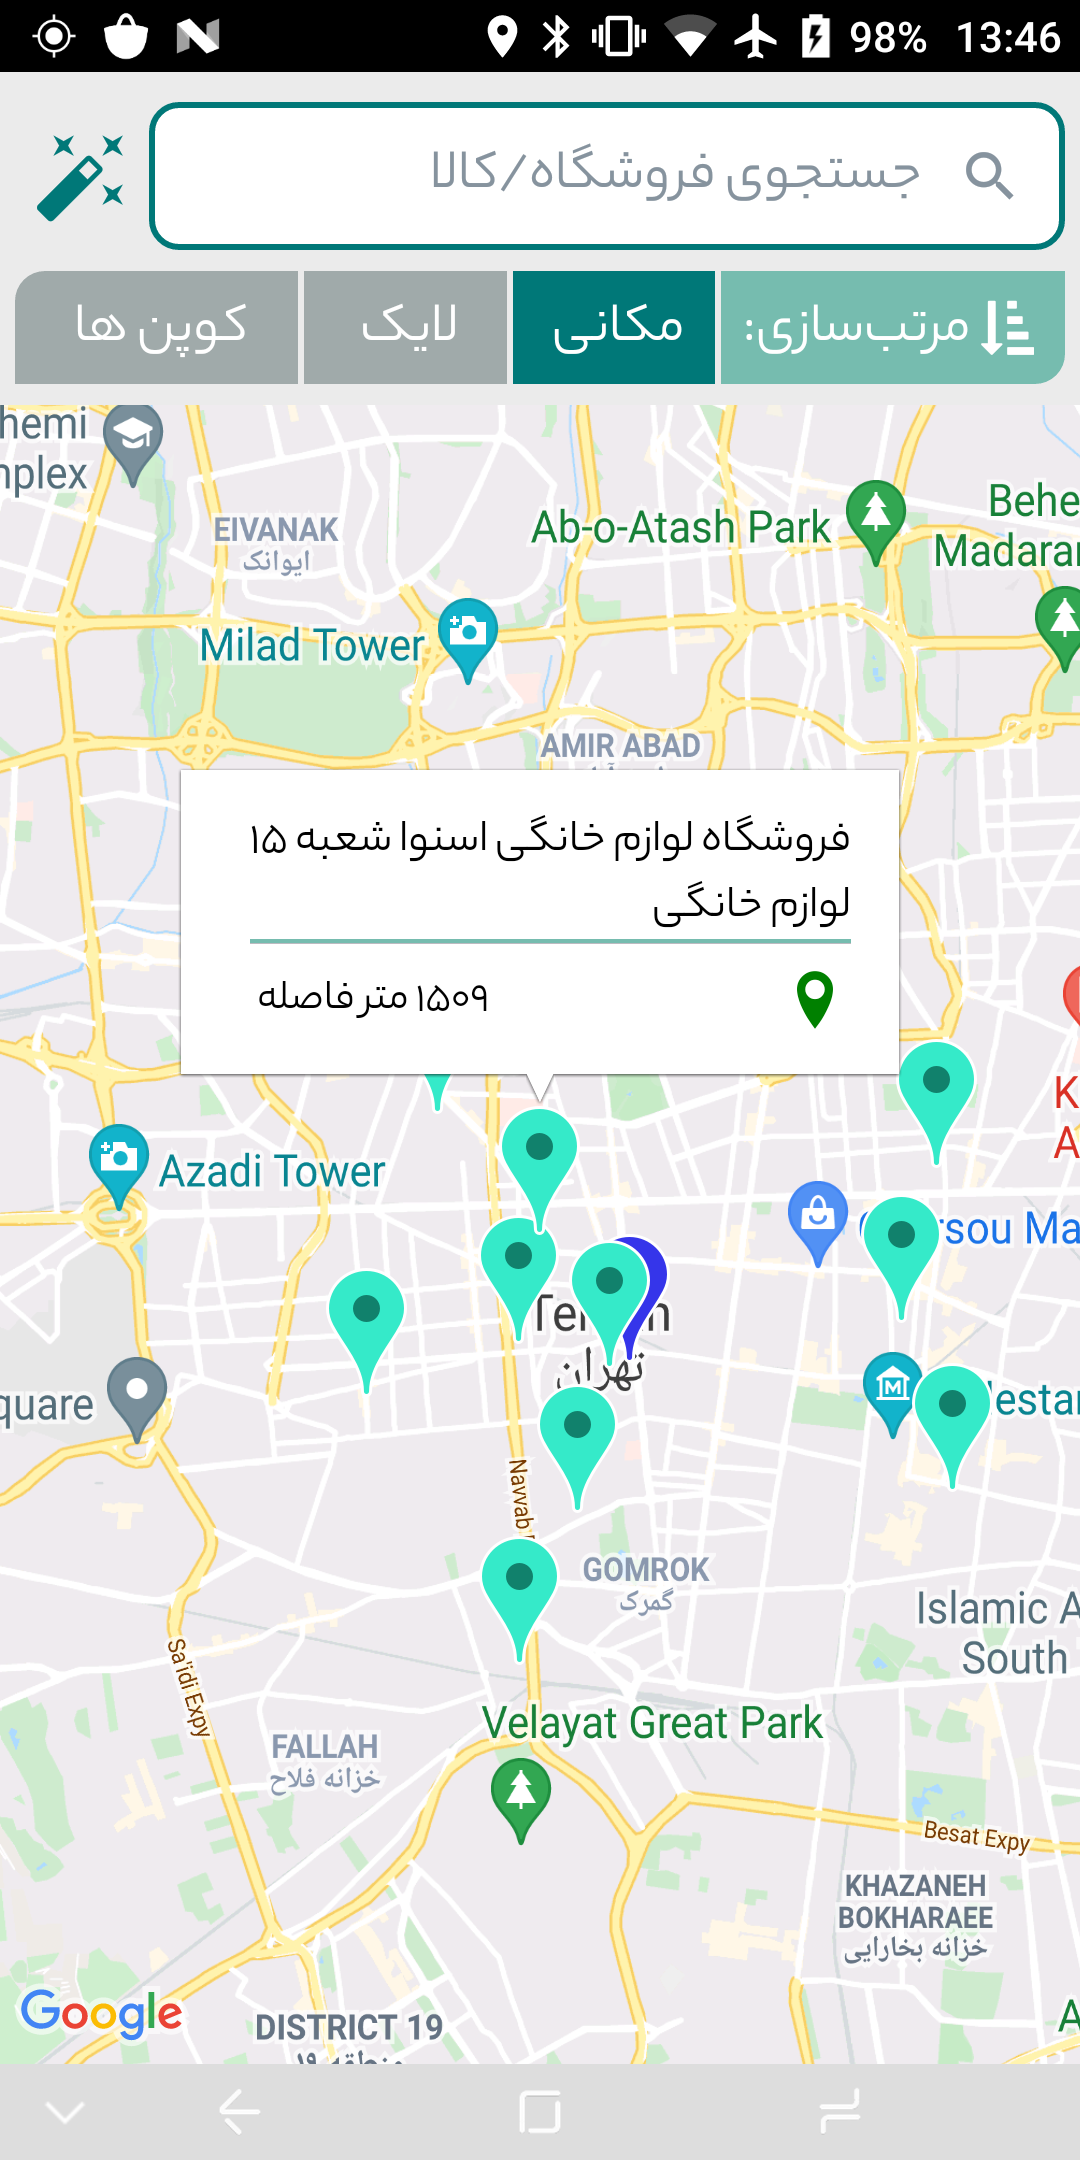
\includegraphics[scale=0.12]{11}
	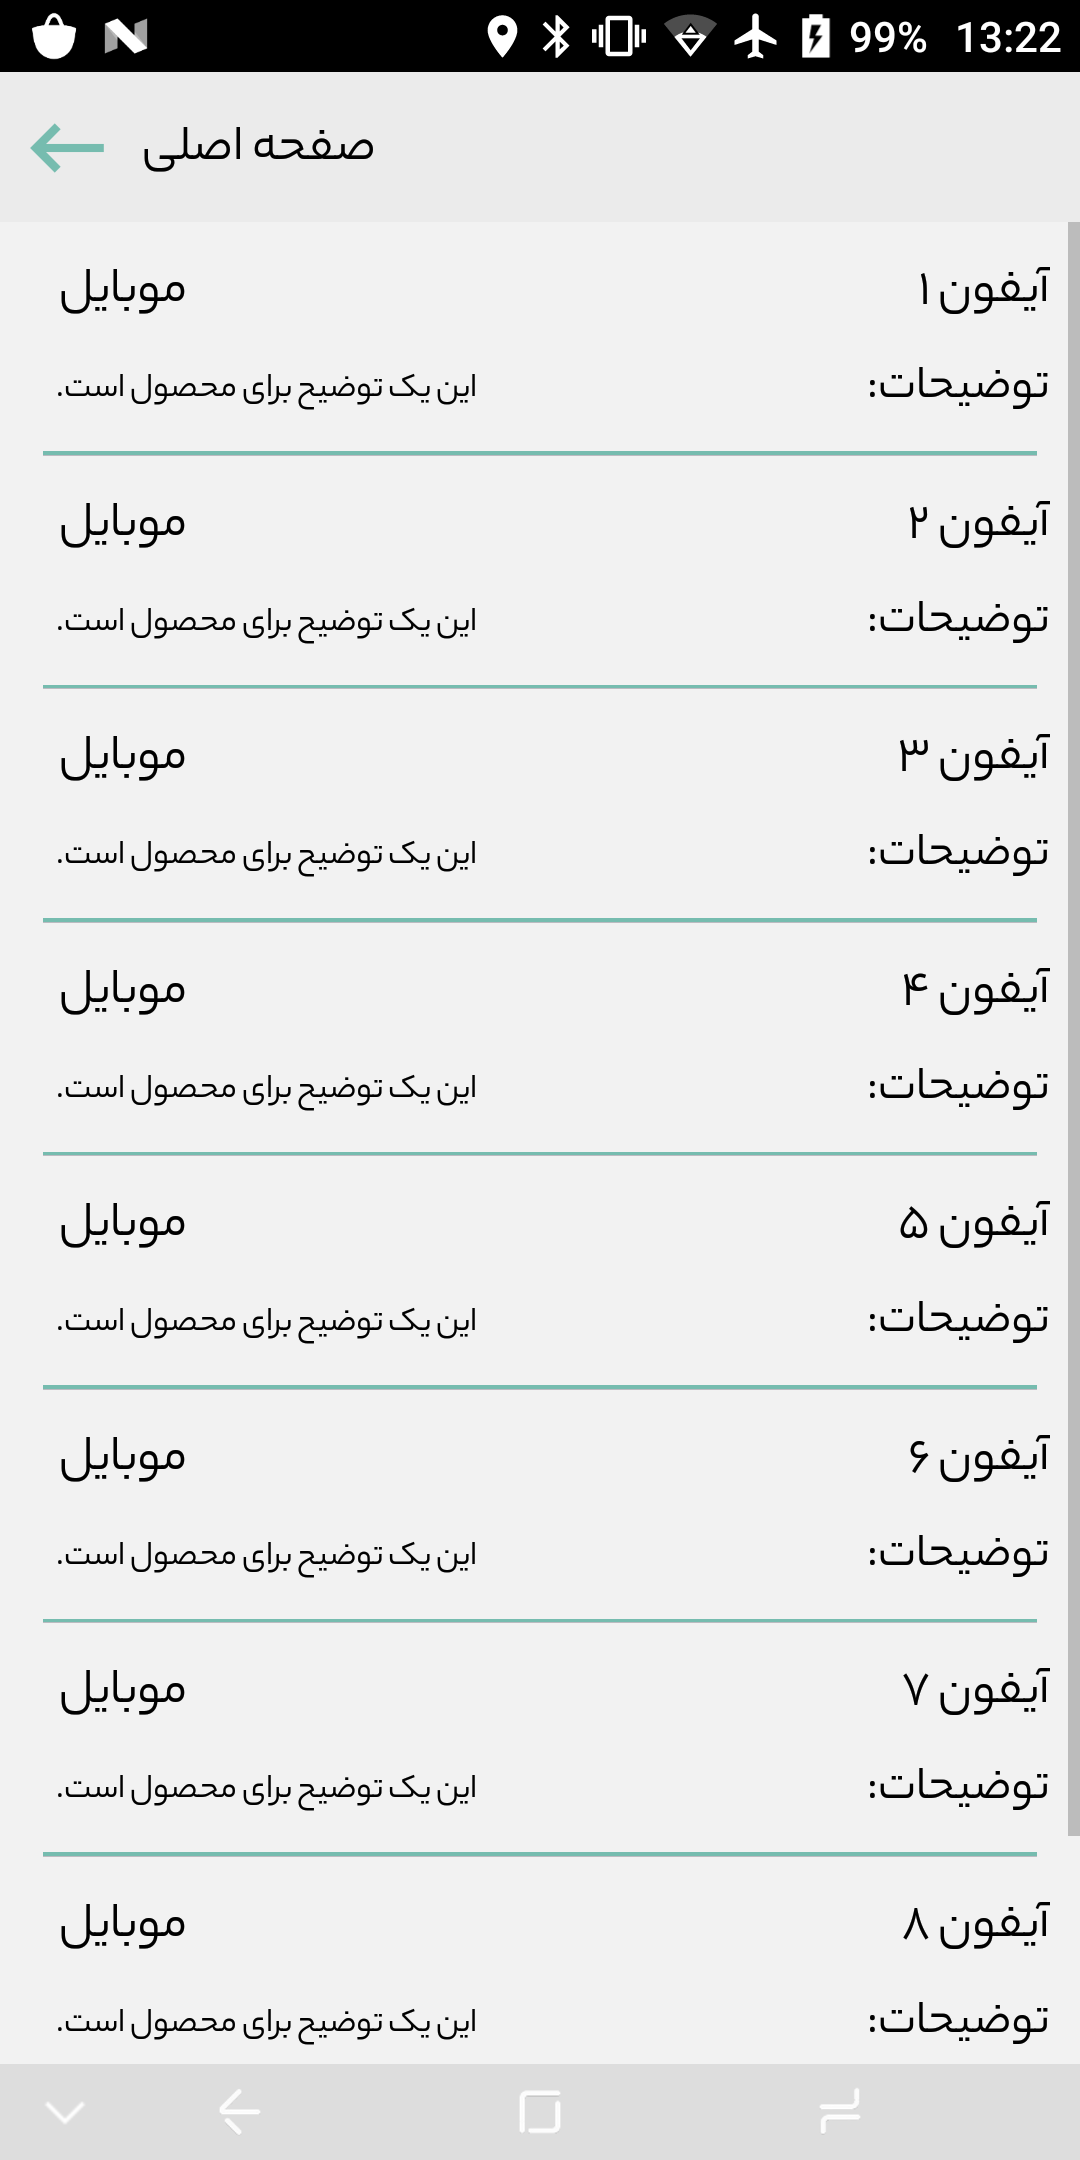
\includegraphics[scale=0.12]{8}
	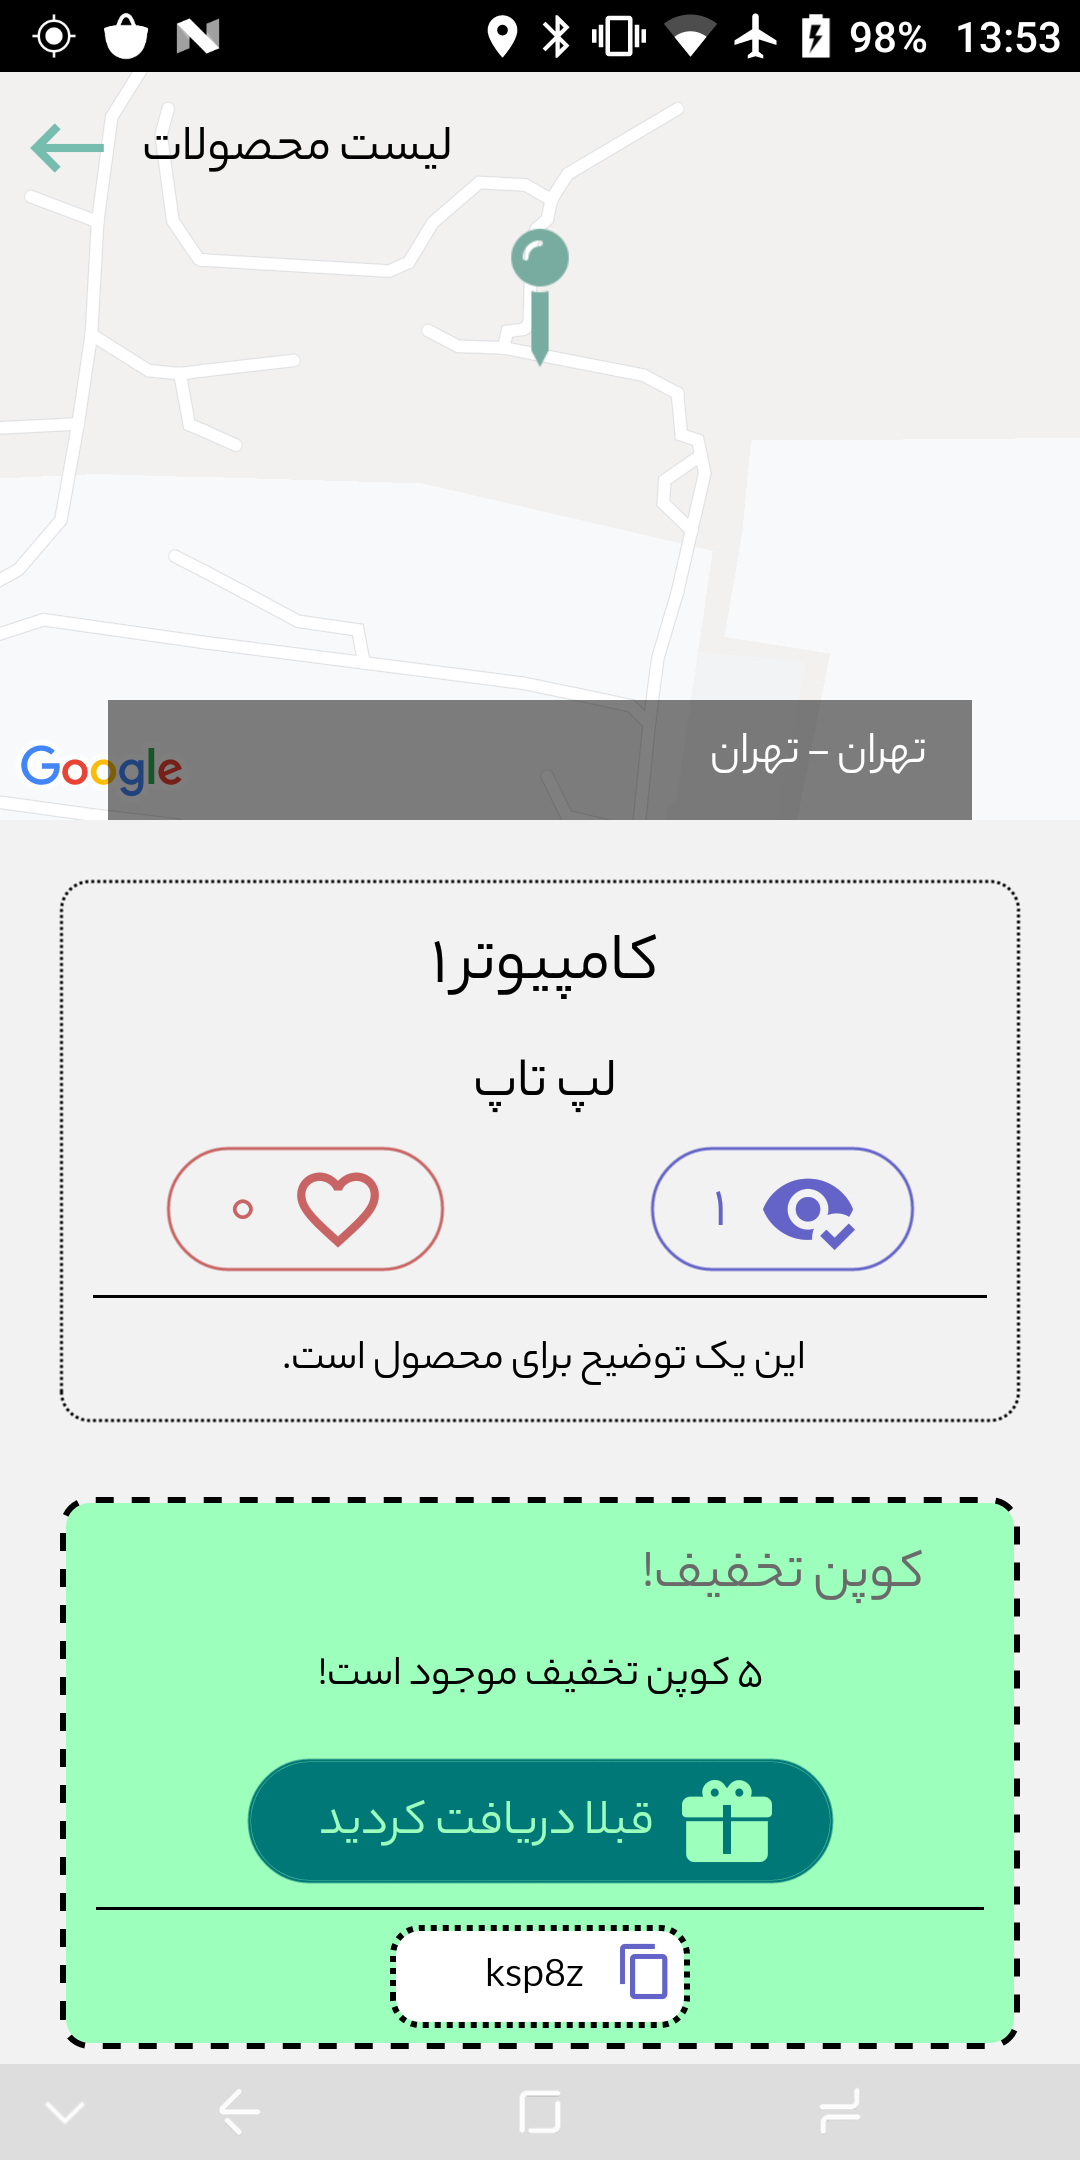
\includegraphics[scale=0.12]{15}
	\caption{به ترتیب از راست، صفحه نقشه فروشگاه‌ها، لیست محصولات یک فروشگاه، صفحه یک محصول}
	\label{fig:app1}
\end{figure}

\begin{figure}[H]
	\centering
	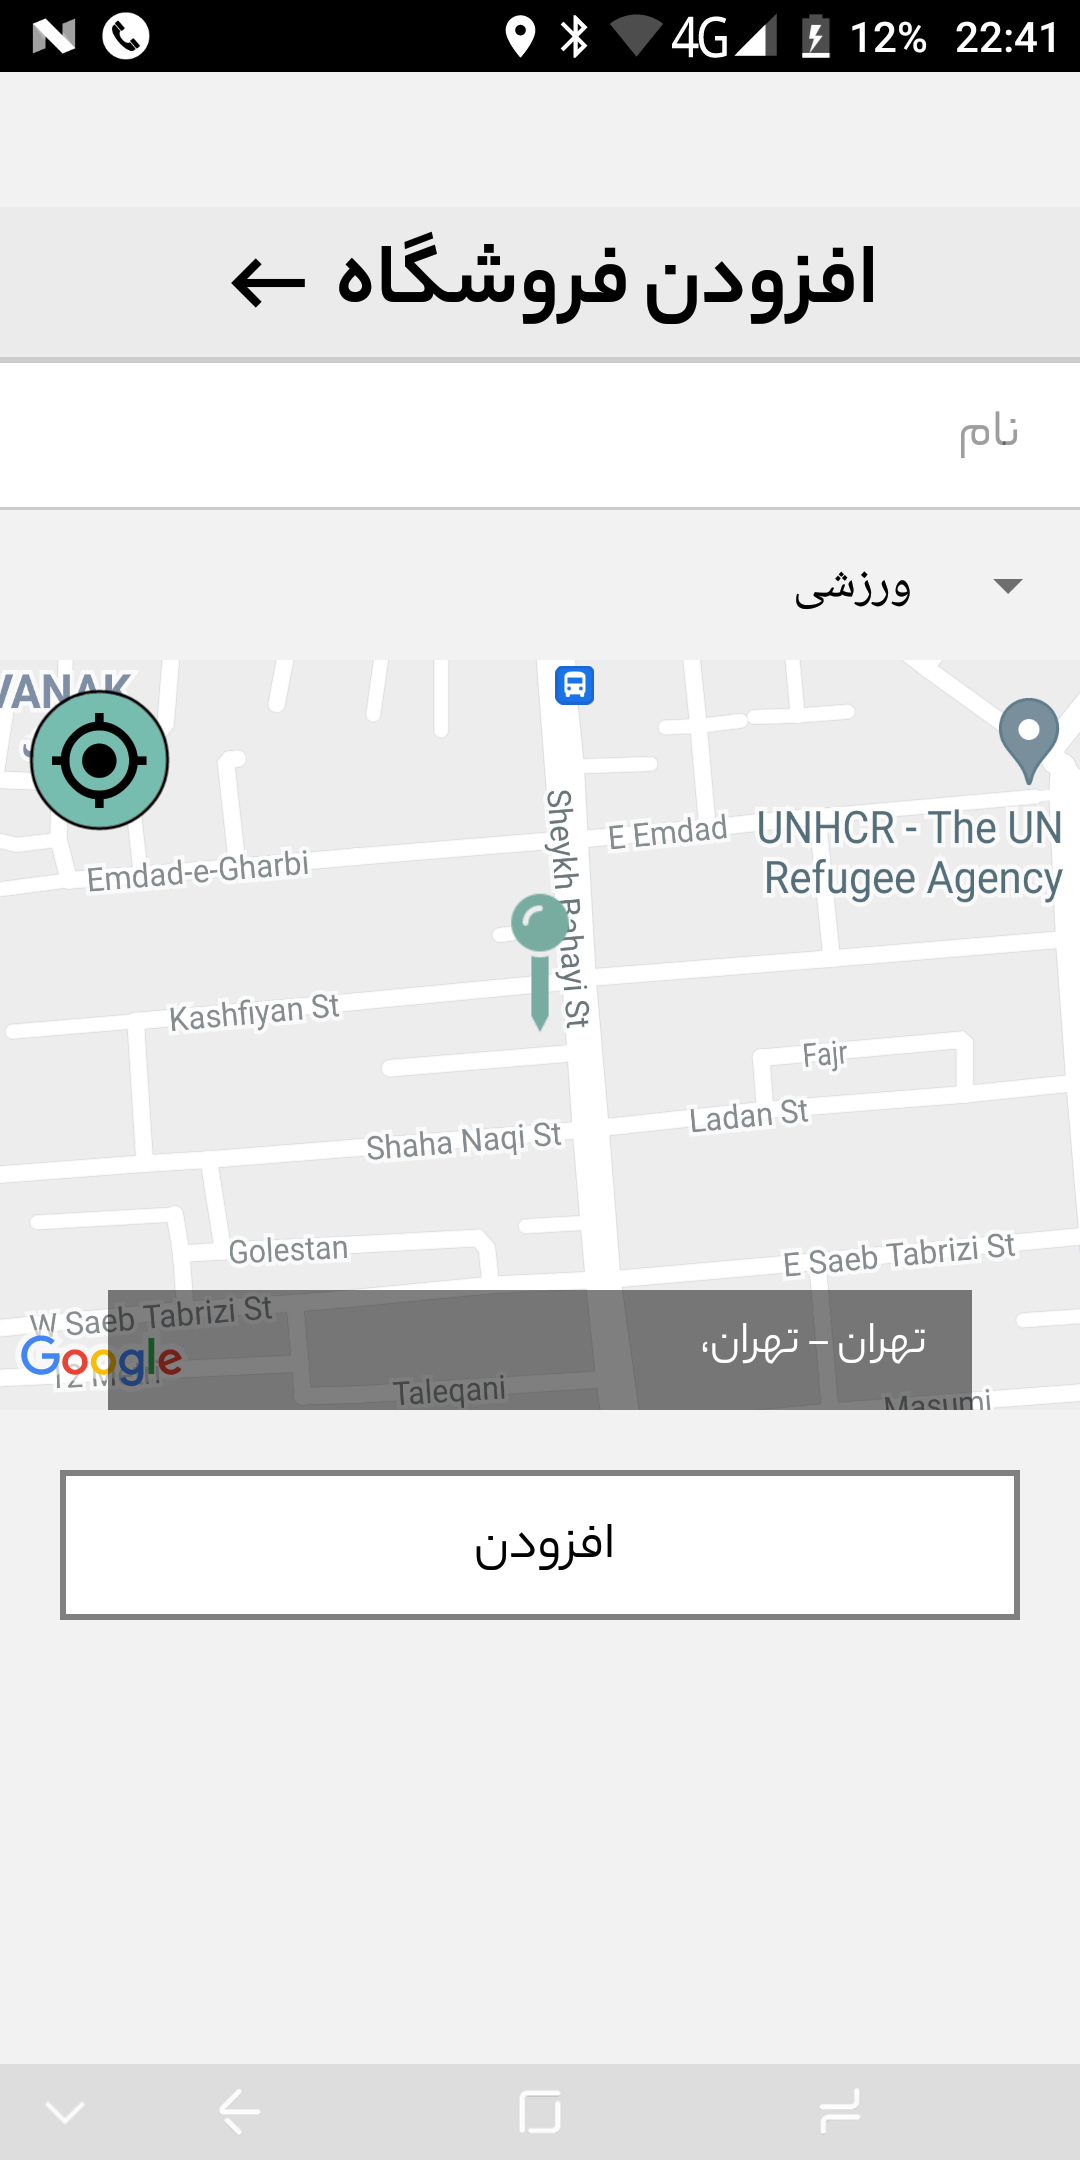
\includegraphics[scale=0.12]{4}
	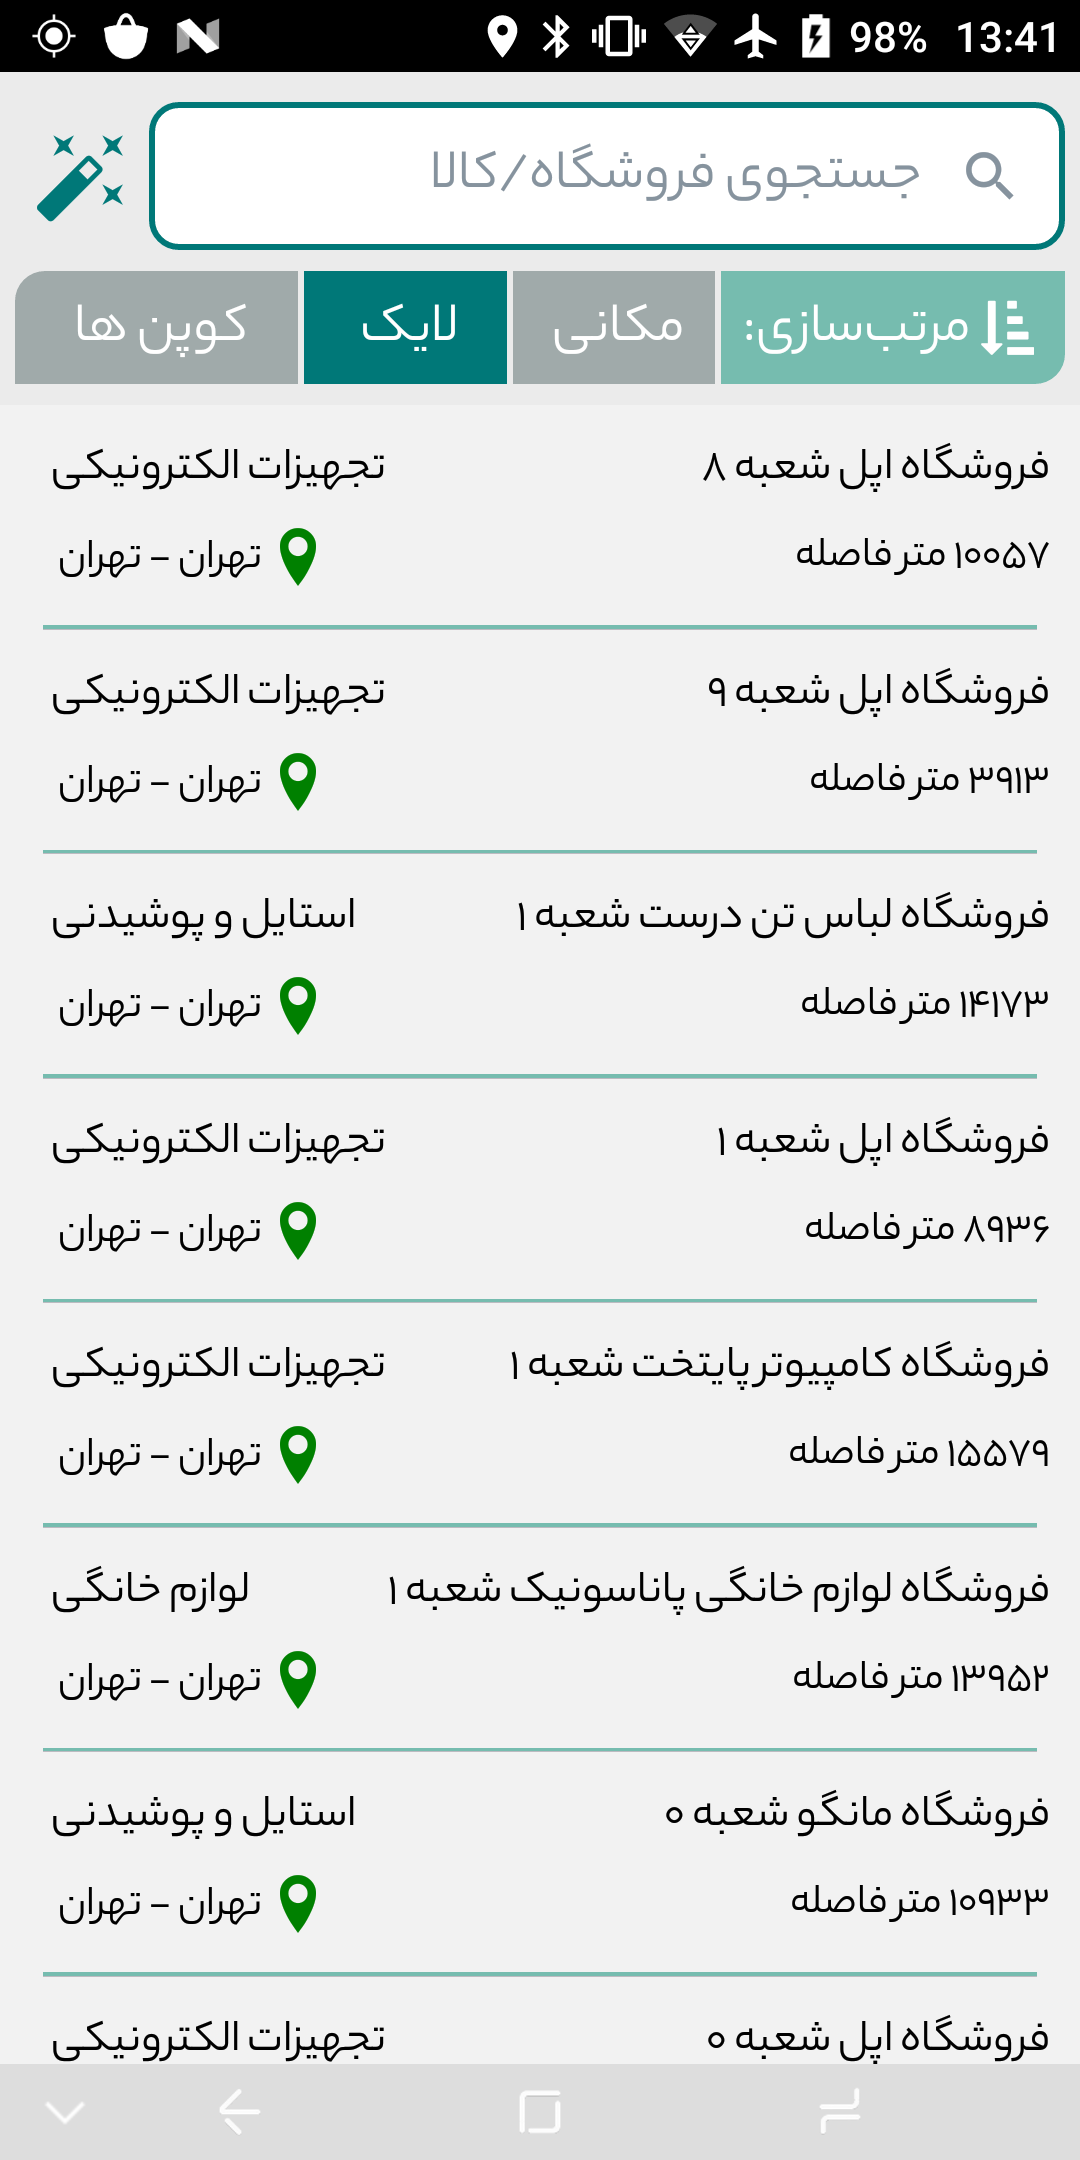
\includegraphics[scale=0.12]{10}
	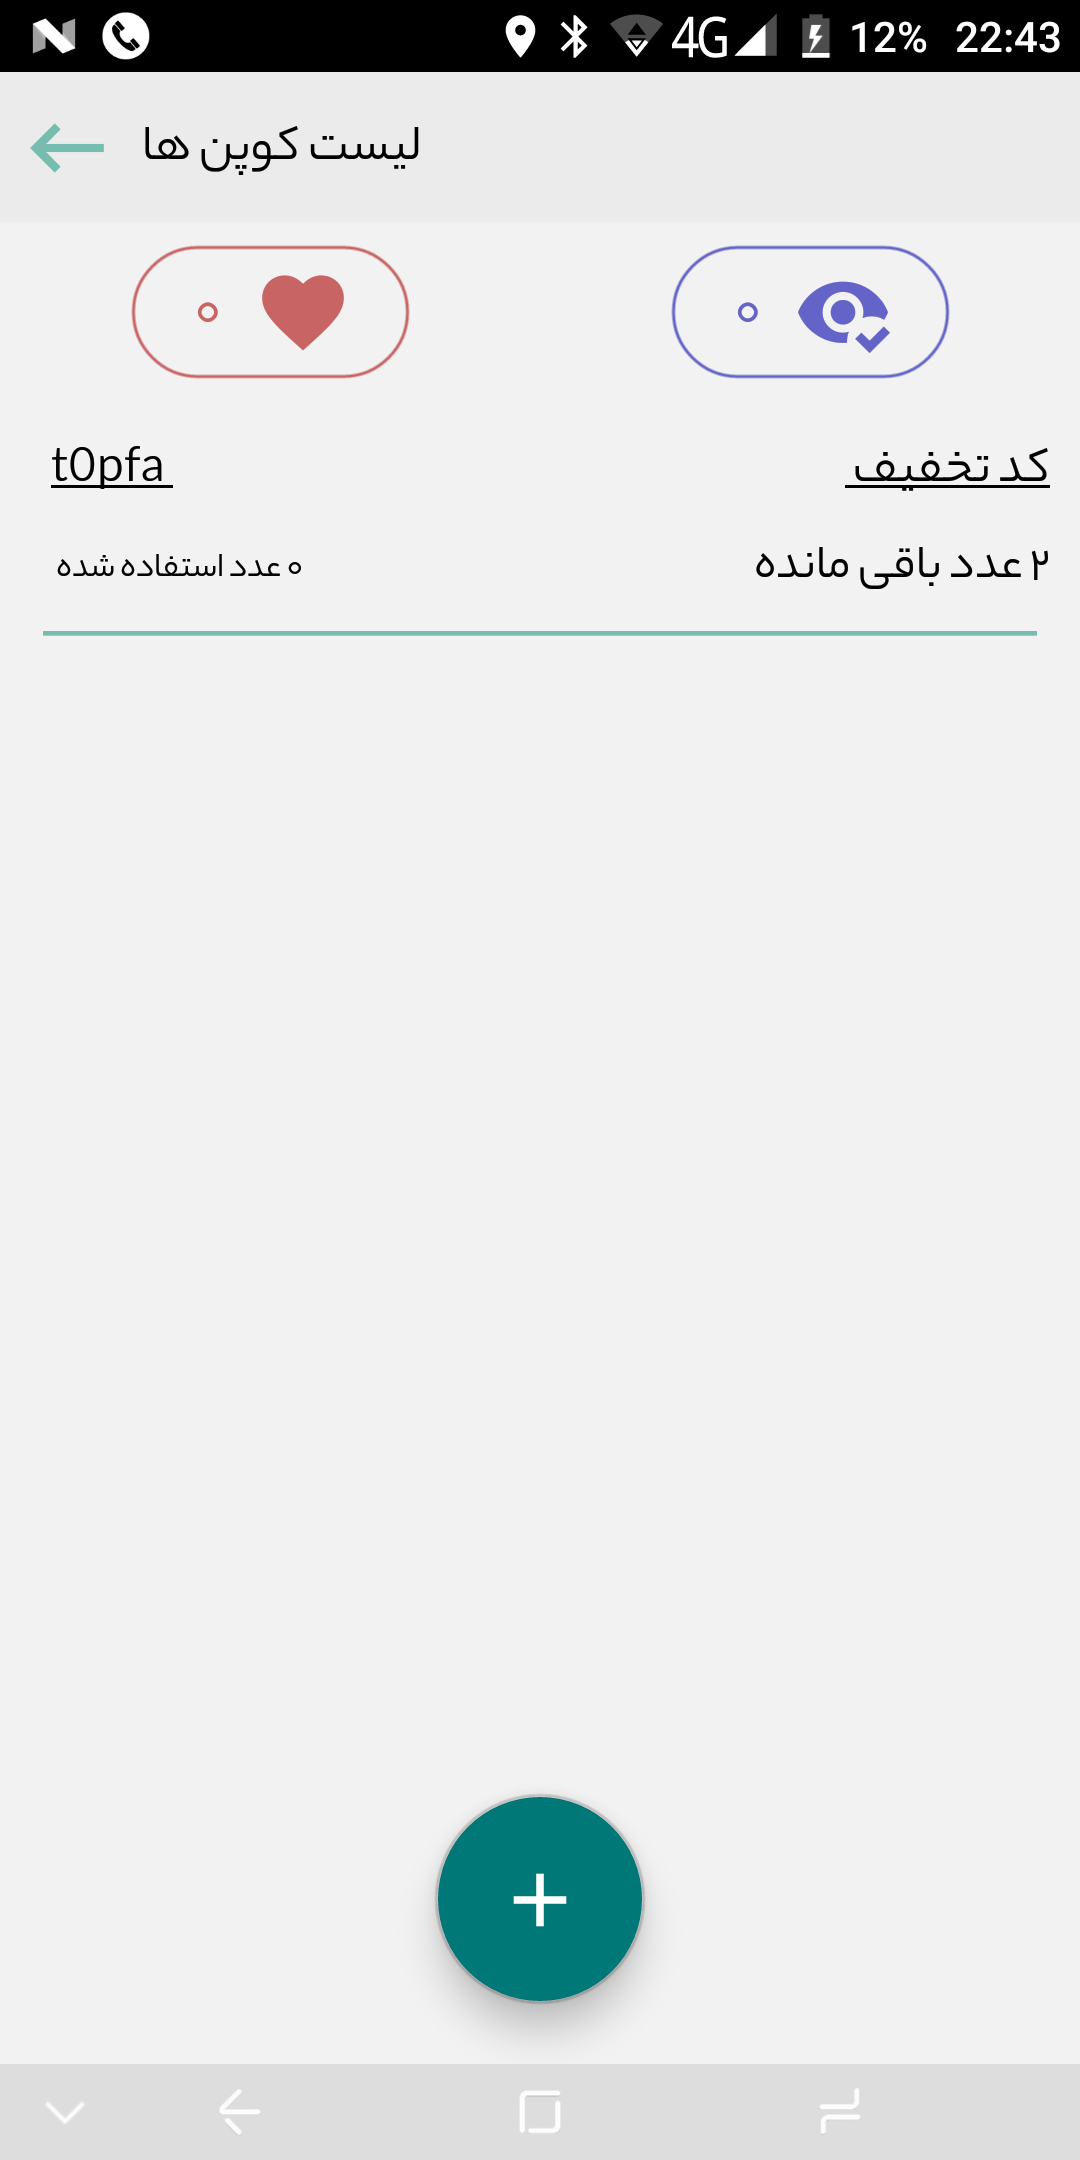
\includegraphics[scale=0.12]{6}
	\caption{به ترتیب از راست، صفحه افزودن فروشگاه، صفحه لیست فروشگاه‌ها، صفحه مشاهده و آمارگیری لیست کوپن‌ها}
	\label{fig:app2}
\end{figure}

%\section{آزمون سامانه}

همان‌طور که پیش‌تر نیز گفته شده بود، برای پیاده‌سازی آزمون‌های خودکار برای این سامانه از ابزار موکا و چای استفاده شده است. این پیاده‌سازی شامل چند بخش می‌شود که در ادامه به آن‌ها خواهیم پرداخت.

%\subsection{تولید داده‌های معتبر جهت آزمون سامانه}

در فصل قبلی نیز توضیح داده شد که حتی برای آزمون دستی سامانه نیز،‌ نیازمند مجموعه وسیعی از داده‌های معتبر ثبت شده درون سامانه خواهد بود. بنابراین بخشی از پیاده‌سازی انجام شده برای آزمون سامانه، به ایجاد و تنظیم  پایگاه‌داده‌ای از اطلاعات مصنوعی ولی معتبر پرداخته است؛ برای مثال در قطعه کد زیر، اطلاعات شخصی کاربران بصورت تصادفی تولید شده و به سامانه اضافه می‌گردد:
\begin{LTR}
	\begin{verbatim}
		await Promise.all(users.map(({token}, i) => {
		    let fname = getRand(FNAMES);
		    let lname = "";
		    do {
		        lname = getRand(LNAMES);
		    } while (pickedNames.includes(fname + " " + lname));
		    pickedNames.push(fname + " " + lname);
			
		    return apolloClient.query({
		        query: UPDATE_UIIS,
		        variables: { fname, lname, gender: "M",
		            birthYear: (i % 50) + 1340, isSalesman: true },
		        context: {
		            headers: { "authorization": `Bearer ${token}` }
		        },
		        fetchPolicy: 'no-cache',
		    }).catch(err => console.log(JSON.stringify(err)));
		}));
	\end{verbatim}
\end{LTR}

%\subsection{آزمون‌های واحد \lr{API}}

این نوع آزمون‌ها شامل آزمون‌های واحد برای \lr{API} سامانه هستند که دقیقا مشابه یک سرویس‌گیرنده به سامانه درخواست می‌دهند و صحت اجرای آن را بررسی می‌کنند که در پیاده‌سازی این آزمون‌ها می‌توان از رویکرد \lr{TDD} استفاده کرد؛ زیرا این آزمون‌ها می‌توانند مستقل از پیاده‌سازی سامانه اصلی ایجاد شوند و طراحی رابط‌های آن را پیش از آن‌که پیاده‌سازی شده باشند مشخص کنند.\\

در این آزمون‌ها بخش‌های مهم‌تر \lr{API} که در بخش‌های قبلی توضیح داده شده بودند مورد بررسی قرار گرفته‌اند که شامل گره اصلی ارائه پیشنهاد، گره‌های دریافت تکی و گره‌های تغییردهنده\footnote{\lr{Modifier}} موجودیت‌های آرایه‌ای پایگاه‌داده (مانند تغییر دادن اطلاعات فروشگاه)، گره‌های مرتبط با احرازهویت و چند گره فرعی دیگر می‌شوند.

%\subsection{آزمون‌های واحد غیر مرتبط با \lr{API}}

این آزمون‌ها برای بررسی صحت برخی از توابع کمکی استفاده شده درون سامانه مورد استفاده قرار گرفته‌اند. مانند توابع خطی‌ساز اشیاء، فیلترهای آرایه، توابع تولید بلیت \lr{JWT} و...؛

\begin{figure}[H]
	\centering
	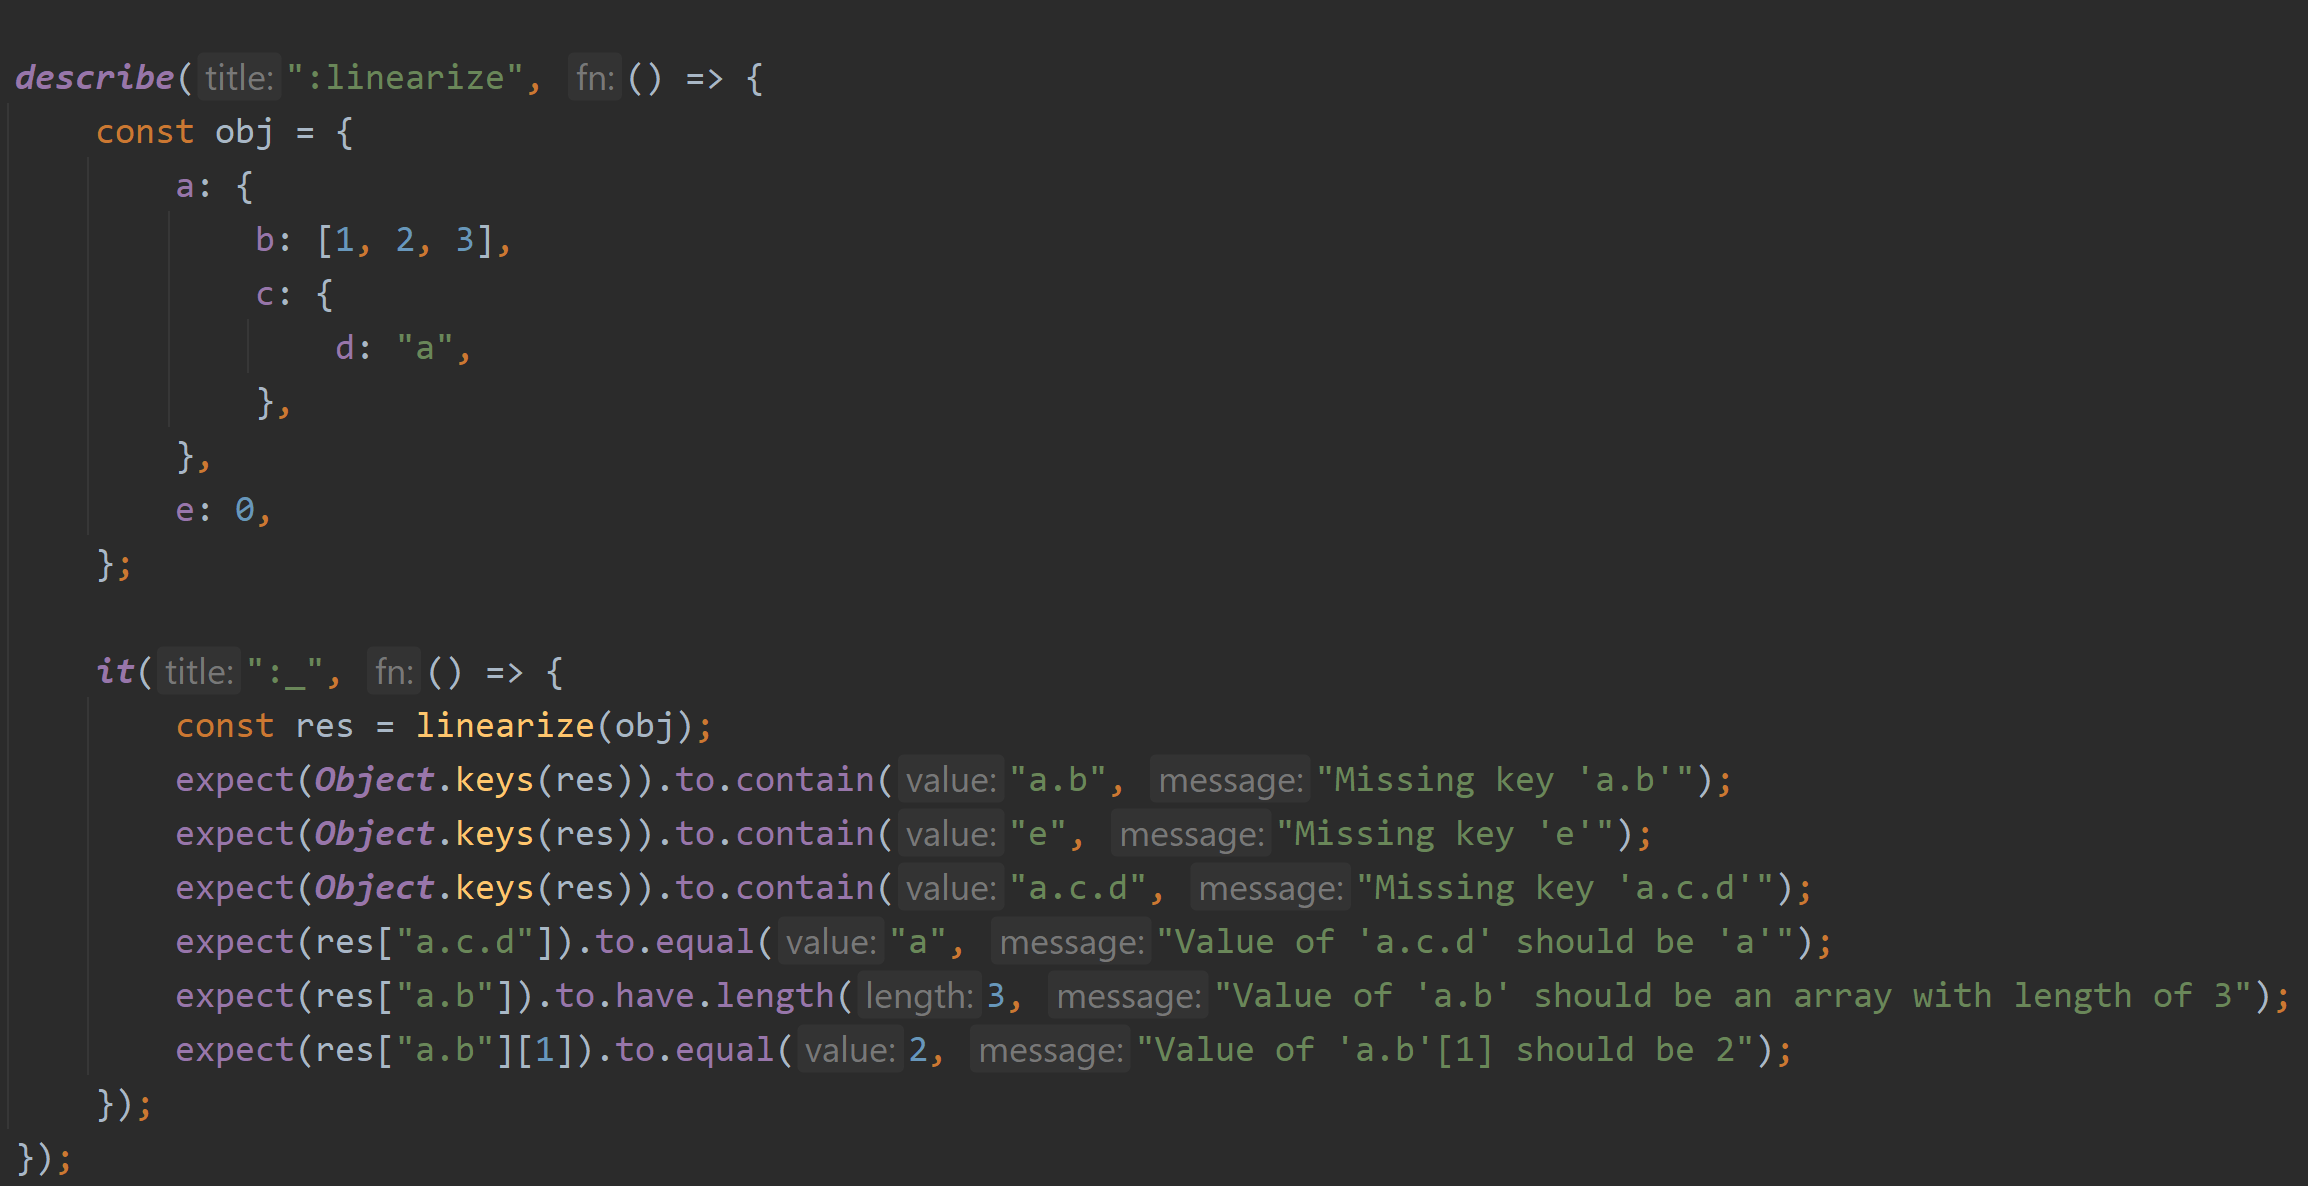
\includegraphics[scale=0.4]{test1}
	\caption{آزمون واحد تابع خطی‌ساز اشیا}
	\label{fig:test1}
\end{figure}

\newpage

آن‌چه در انتهای \cref{fig:test1} نوشته شده، دستورات کتابخانه چای است که با رویکرد \lr{BDD} استفاده شده است. درواقع در این رویکرد، انتظارات ما از نتیجه اجرای یک بخش از کد که مورد آزمون قرار گرفته است، بصورت رفتاری توصیف می‌شود و همان‌طور که در این شکل نیز مشخص است، توابع این کتابخانه مانند اجزای یک جمله انگلیسی به یکدیگر متصل شده و عملا هر یک از آن جملات درحال توصیف یک انتظار ما از رفتار تابع \lr{linearize} هستند.

\begin{figure}[H]
	\centering
	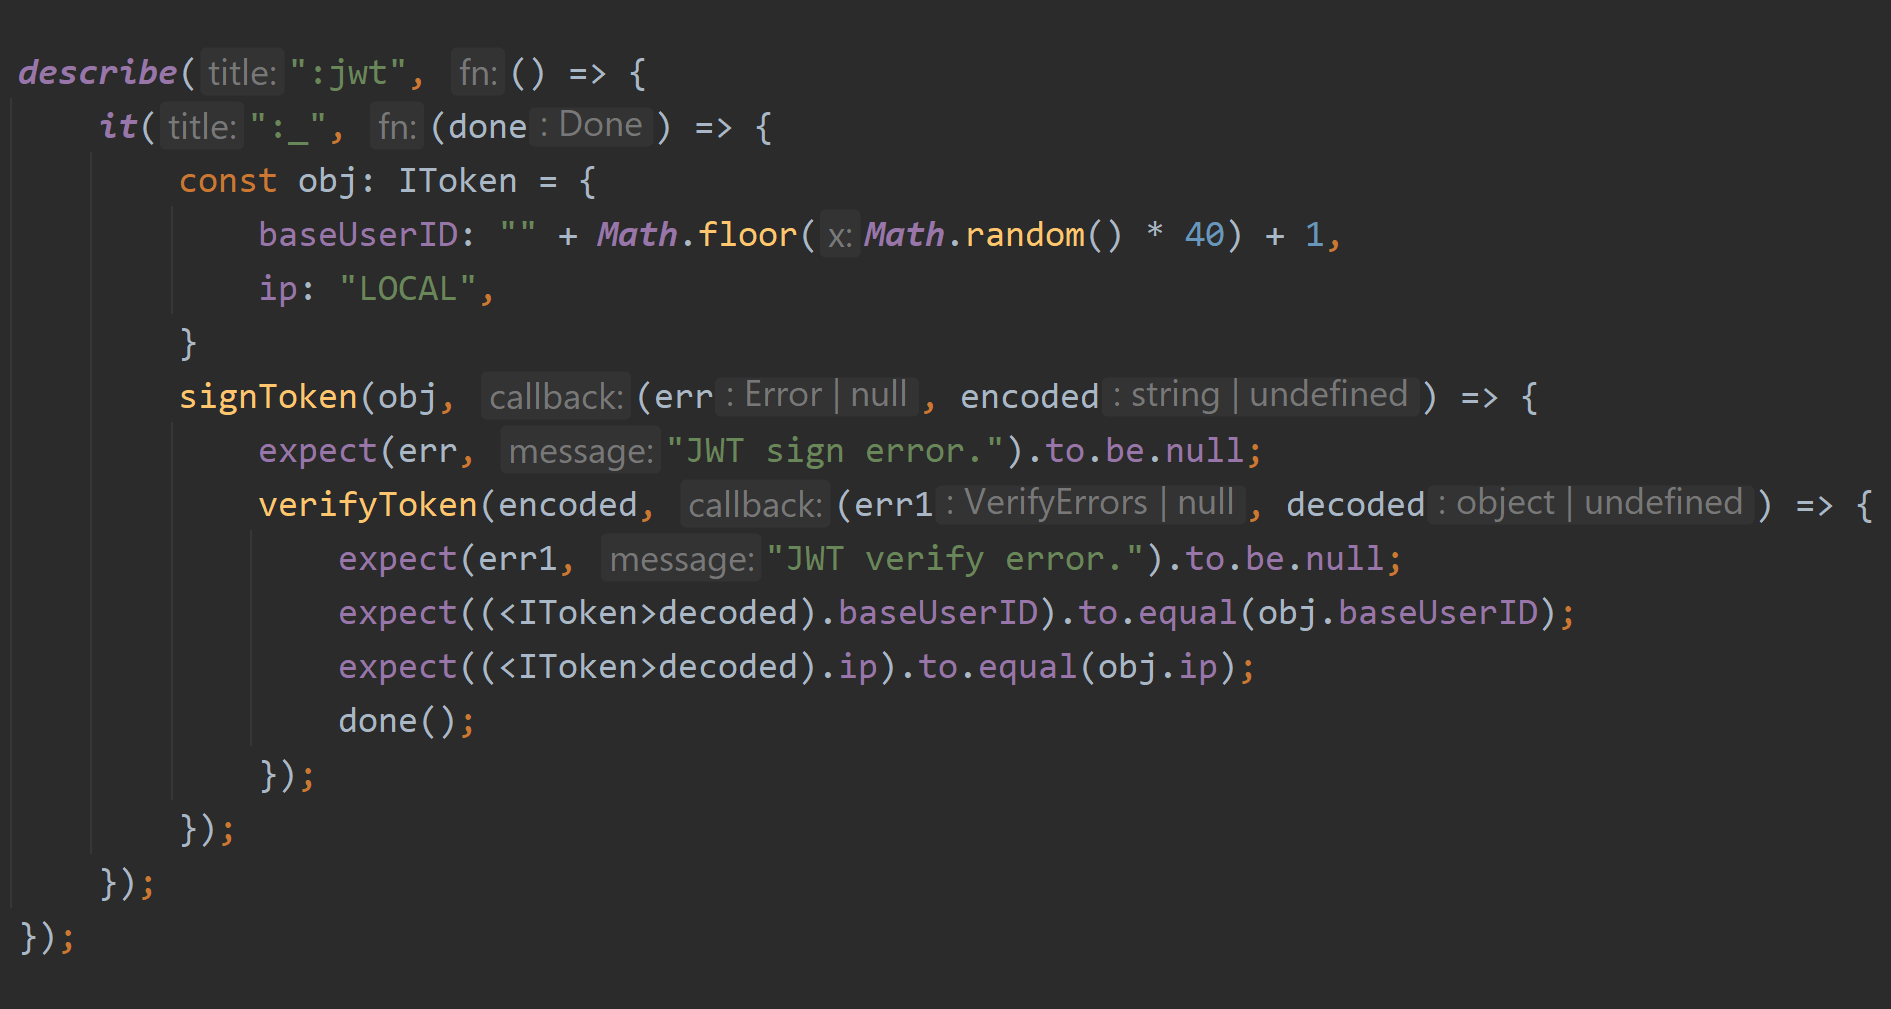
\includegraphics[scale=0.45]{test2}
	\caption{آزمون واحد تولید بلیت با \lr{JWT}}
	\label{fig:test2}
\end{figure}

	در \cref{fig:test2} نیز نمونه‌ای دیگر از آزمون‌های واحد برای بررسی صحت عملکرد تولیدکننده بلیت احراز هویت \lr{JWT} نمایش داده شده که در این‌جا نیز از ساختار \lr{BDD} کتابخانه چای استفاده گردیده است.

%\subsection{آزمون استرس‌پذیری سامانه}

این آزمون با استفاده از سامانه \lr{K6}\cite{k6} انجام شده که یکی از سامانه‌های بسیار معروف برای انجام تست‌های بار\footnote{\lr{Load Test}} بر روی سامانه‌های ارائه‌دهنده \lr{API} است.

نمودار خروجی یکی از این آزمون‌ها در \cref{fig:test4} قابل مشاهده است. این آزمون با مجموع 4383 درخواست فشرده (با 30 کاربر مجازی همزمان که در طول 3 دقیقه و 30 ثانیه مدت تست بصورت خطی فعالیت خود را شروع کرده‌اند) که هرکدام از آن‌ها شامل 4 درخواست داخلی است انجام شده (یعنی در مجموع 17532 درخواست) که در نتیجه‌ی آن، هیچ‌گونه اختلال عملکرد در سرویس‌دهی به این درخواست‌ها مشاهده نشده و میانگین مدت زمان پاسخ ارائه‌دهنده سرویس 154 میلی‌ثانیه ثبت شده است. لازم به ذکر است که درخواست‌های ایجاد شده برای این تست بار، از پیچیده‌ترین درخواست‌های ممکن برای این سامانه تشکیل شده‌اند و در سامانه واقعی اکثر درخواست‌ها سطح پیچیدگی بسیار پایین‌تری دارند.\\

مشخصات اجرایی این سامانه در آزمون بار انجام شده به این صورت بوده است:
\begin{itemize}
	\item پایگاه داده مونگو
	\begin{enumerate}
		\item پردازنده: 20 درصد از یک هسته
		\item حافظه اصلی: 300 مگابایت
	\end{enumerate}
	\item سامانه اصلی
	\begin{enumerate}
		\item پردازنده: 25 درصد از یک هسته
		\item حافظه اصلی: 250 مگابایت
	\end{enumerate}
\end{itemize}

\begin{figure}[H]
	\centering
	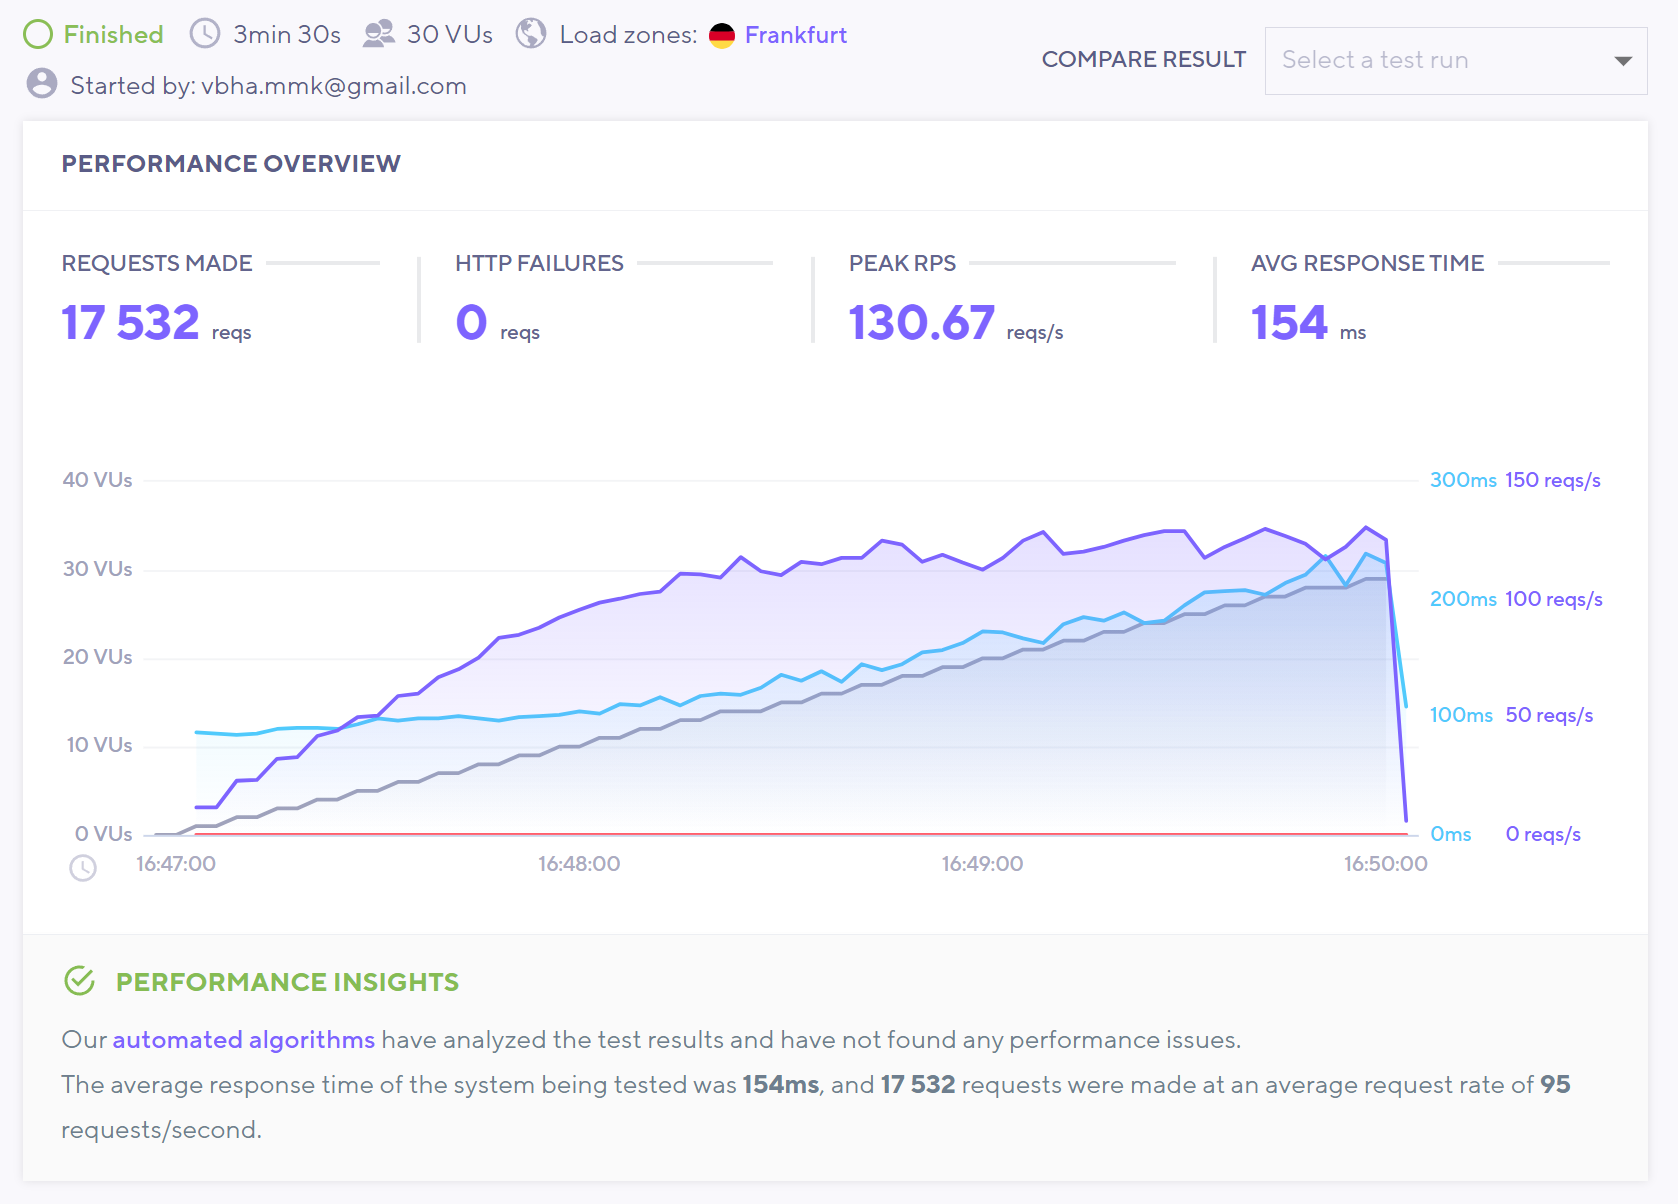
\includegraphics[scale=0.53]{test4}
	\caption{آزمون بار توسط سامانه \lr{K6}}
	\label{fig:test4}
\end{figure}

در توضیح رنگ‌های استفاده شده در نمودار \cref{fig:test4}، رنگ خاکستری (که در محور سمت چپ قابل مشاهده است) بیانگر تعداد واحدهای مجازی است که در هرلحظه بصورت همزمان درحال ارسال درخواست به سمت سامانه بوده‌اند. تعداد این کاربران مجازی در حداکثر حالت رایگان مجاز در این ابزار‌ (یعنی 30 کاربر همزمان) تنظیم شده است که از ابتدای شروع آزمون بصورت خطی افزایش پیدا کرده و به عدد 30 رسیده است.

رنگ آبی مدت زمان پاسخ سامانه می‌باشد که از حدود 100 میلی‌ثانیه شروع شده و در نهایت به حدود 220 میلی‌ثانیه ختم شده است. همچنین رنگ بنفش نشان دهنده تعداد درخواست‌های پاسخ داده شده در هر لحظه است؛ در ثانیه‌های ابتدای تست اعداد رنگ آبی و بنفش نمایش داده نشده‌اند، زیرا مدت زمانی طول می‌کشد تا اولین درخواست پاسخ داده شود و پیش از آن این دو مقدار قابل محاسبه نخواهند بود؛ رنگ قرمز نیز تعداد درخواست‌های ناموفق را نشان می‌دهد که در اینجا همواره صفر بوده است و تمامی درخواست‌ها با موفقیت پاسخ داده شده‌اند.

آن‌چیزی که از این نمودار می‌توان برداشت کرد این است که از حدود \lr{VU = 12} به بعد، مقدار نمودار رنگ آبی (زمان پاسخ) نرخ افزایش بیشتری داشته و برعکس، نرخ پاسخ‌دهی به درخواست‌ها (نمودار بنفش رنگ) صعود چشمگیری نداشته است. درواقع با این‌که این سامانه قابلیت پاسخگویی با تاخیر منطقی و استانداردی (زیر 250 میلی‌ثانیه) را حتی برای 30 کاربر همزمان با 17 هزار درخواست پیچیده داشته است، اما بهترین تاخیر، حداکثر برای 12 کاربر همزمان اتفاق افتاده است. البته باید توجه داشت که این 12 کاربر هر کدام و در هر ثانیه درحال ارسال 4 درخواست پیچیده و بصورت همزمان بوده‌اند که هر یک از آن‌ها از 4 درخواست درونی تشکیل شده‌اند؛ بنابراین تعداد کاربران واقعی برای وضعیت گفته شده حداقل 4 برابر مقدار ذکر شده، یعنی 48 کاربر خواهد بود.
